\mysection{エミッタ接地回路のバイアス電圧$v_{be}$の設定}
エミッタ接地回路の動作点設定を、原理の説明とシミュレーションによる演習により理解する。

\begin{description}
  \setlength{\parskip}{0cm} % 段落間
  \setlength{\itemsep}{0cm} % 項目間
  \item[ゴール] 2電源バイアス回路をLTSpiceで設計する。(バイアス電圧$V_{be}$と負荷抵抗$R_L$を決定する。)
  \item[キーワード] $I_C$-$V_{CE}$特性、$I_E$-$V_{BE}$ 特性、負荷線、動作点 $V_{CEO}$・$I_{CO}$・$V_{BEO}$
  \item[ストーリー] $I_E$-$V_{BE}$特性と、$I_C$-$V_{CE}$特性を使って、動作点 $V_{CEO}$・$I_{CO}$・$V_{BEO}$ を決める。→ 過渡解析により増幅率を実測 → 計算値と比較。
\end{description}

\mysubsection{演習手順}
原理で計算した値を用いて図\ref{2den_kaiseki}(a)に示す回路図を設計する。入力信号は正弦波$v_{be} = 5.27$ mVp-p を使用する。

\begin{figure}[htb]
  \begin{center}
  \subfigure[2電源バイアス回路の動作点]{	% 副題なし
  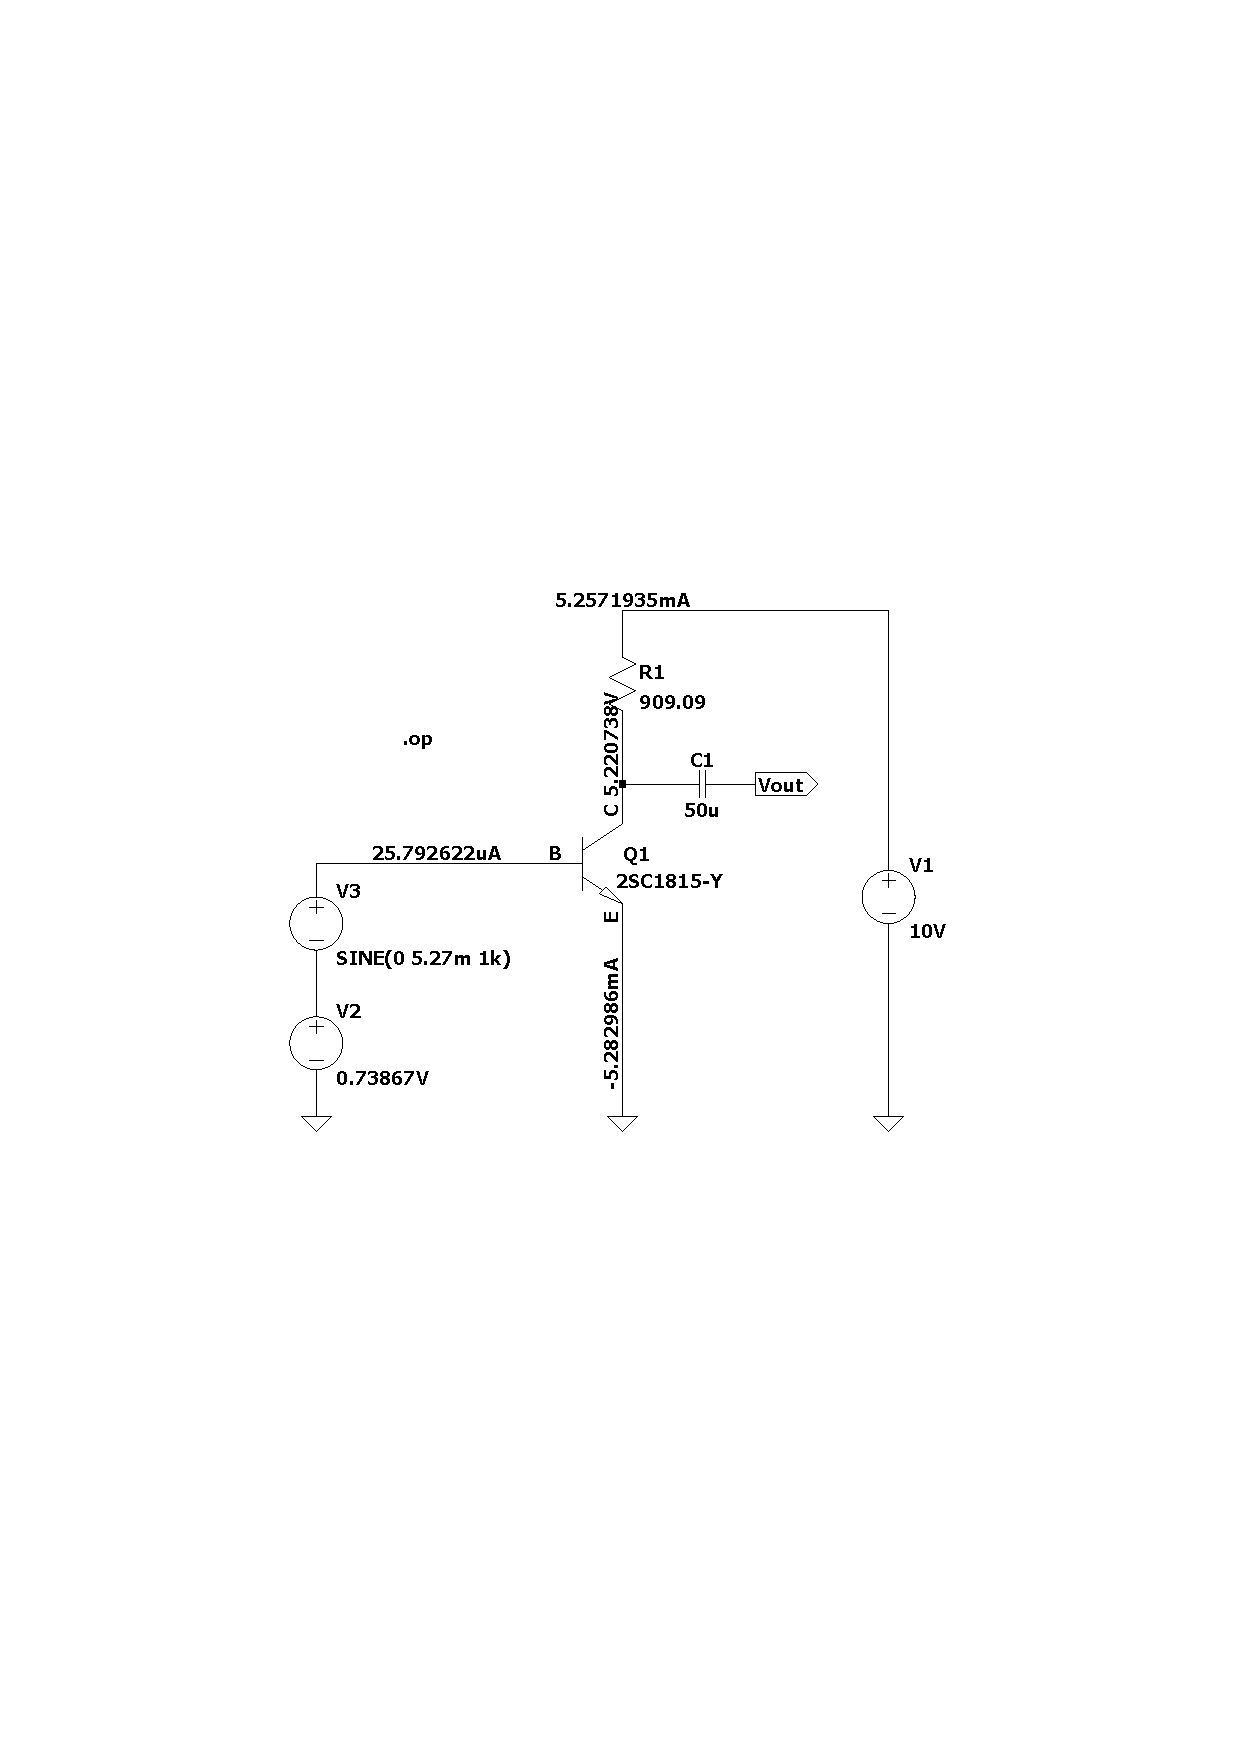
\includegraphics[width=.5\columnwidth]{img/40.pdf}
  }~
  \subfigure[動作点解析結果]{
  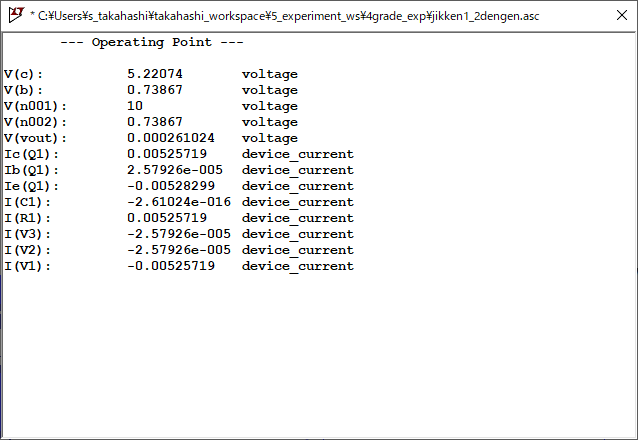
\includegraphics[width=.5\columnwidth]{img/41.png}
  }
  \subfigure[過渡解析結果]{
  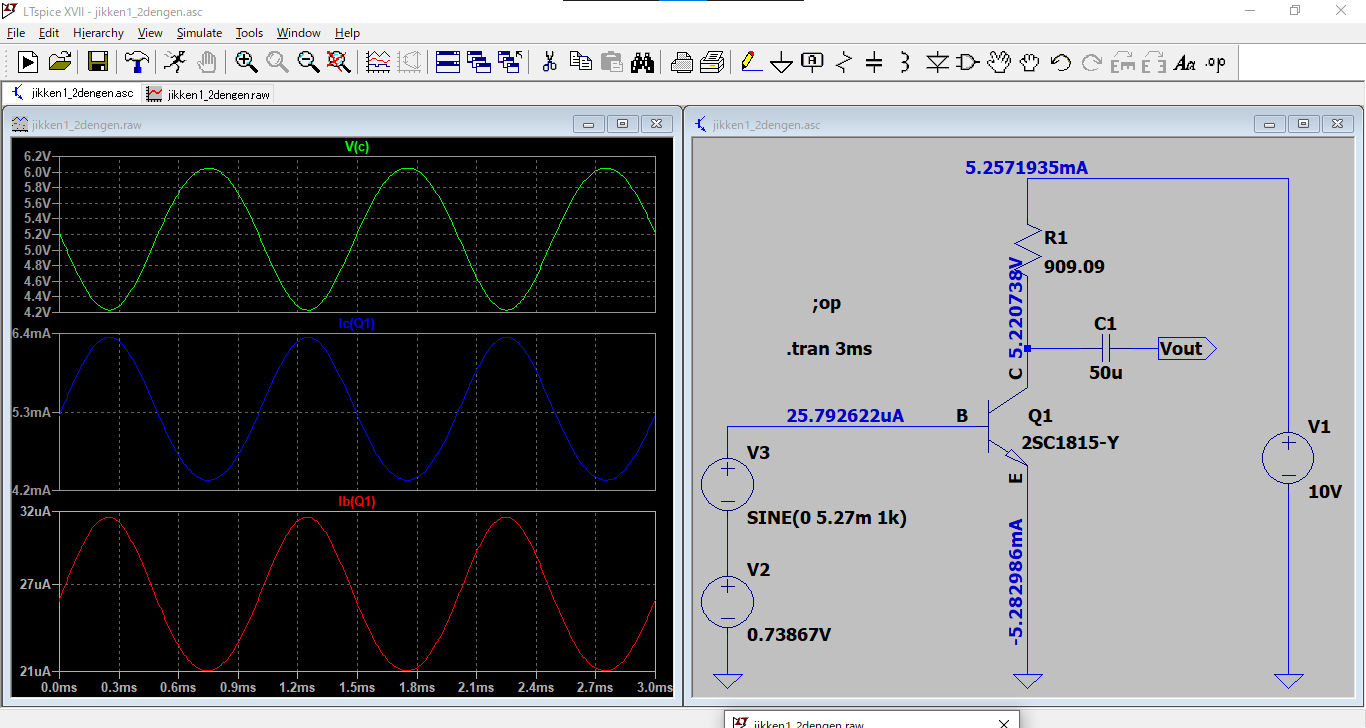
\includegraphics[width=.8\columnwidth]{img/42.png}
  }
  \caption{2電源バイアス回路の各種特性}
  \label{2den_kaiseki}
  \end{center}
\end{figure}

\mysubsubsection{DC動作点解析}
spiceディレクティブ「DC op pnt」に ".op" のみ記述し、ディレクティブに張り付ける → 「Run」で実行。→ 設計した値に対応するベース電流、コレクタ電流がDC動作点の解析結果として現れる。

\begin{description}
  \setlength{\parskip}{0cm} % 段落間
  \setlength{\itemsep}{0cm} % 項目間
  \item[課題5] 2SC1815のDC動作点解析を行ってください。
  (ベース電流、コレクタ電流のDC動作点を求める。)(用いた回路図とディレクティブを示すこと。図\ref{2den_kaiseki}(a)(b))
  動作点が正しく設定されているかどうか根拠と共に説明してください。
  直流電流増幅率$\beta_0$を求めて、計算値と比較して下さい。
\end{description}

\mysubsubsection{過渡解析}
「Edit Simulation cmd.」から Transient 解析を選び、「.tran 3ms」ディレクティブを適用させて、過渡解析を実行する。
この時、$V_C、I_C、I_B$ の波形を確認する。


\begin{description}
  \setlength{\parskip}{0cm} % 段落間
  \setlength{\itemsep}{0cm} % 項目間
  \item [課題6] 2SC1815の過渡解析を行ってください。(用いた回路図とディレクティブを示すこと。図\ref{2den_kaiseki}(c))
  $i_b$、$i_c$の波形に対する、$V_{c}$の波形の位相の特徴を説明して下さい。
  交流電流増幅率 $\beta_0$ を求めて下さい。($\beta_0 = i_c/i_b$)
\end{description}